\begin{minipage}{.3\textwidth}
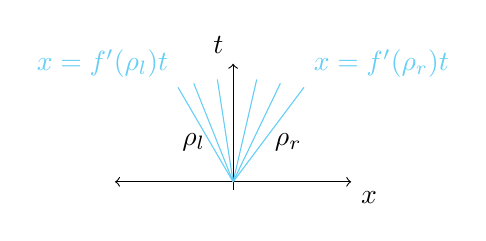
\begin{tikzpicture}
% coord.
\draw[<->] (-1.5,0) -- (1.5,0) node[anchor= north west] {$x$};
\draw[->] (0,-0.1) -- (0,1.5) node[anchor=south east] {$t$};
% rarefaction
\draw[color=cyan!60!white] (0,0) -- (0.9,1.2) node[anchor= south west] {$x = f'(\rho_r)t$};
\draw[color=cyan!60!white] (0,0) -- (0.6,1.25);
\draw[color=cyan!60!white] (0,0) -- (0.3,1.3);
\draw[color=cyan!60!white] (0,0) -- (-0.2,1.3);
\draw[color=cyan!60!white] (0,0) -- (-0.5,1.25);
\draw[color=cyan!60!white] (0,0) -- (-0.7,1.2) node[anchor= south east] {$x = f'(\rho_l)t$};
\node at (-0.5, 0.5) {$\rho_l$};
\node at (0.7, 0.5) {$\rho_r$};
\end{tikzpicture}
\caption{The solution to the Riemann problem, $\rho_l > \rho_r$.}
\label{Fig: SolRP_raref}
\end{minipage}
\quad \quad \quad \quad \quad \quad \quad \quad
\begin{minipage}{.3\textwidth}
\begin{tikzpicture}
\draw[<->] (-1.5,0) -- (1.5,0) node[anchor= north west] {$x$};
\draw[->] (0,-0.1) -- (0,1.5) node[anchor=south east] {$t$};
\draw[color=cyan!90!white] (0,0) -- (0.9,1.2) node[anchor= south west] {$x = st$};
\node at (-0.5, 0.5) {$\rho_l$};
\node at (0.7, 0.5) {$\rho_r$};
\end{tikzpicture}
\caption{The solution to the Riemann problem, $\rho_l < \rho_r$.}
\label{Fig: SolRP_shock}
\end{minipage}